\subsection*{Separating earned evidence from messages changes when communication is useful}
The candidate rule maintains signed evidence and confidence in two distinct pairs of fields (Fig.~\ref{fig:local-evidence}): one records the unit's own completed contacts, while the other carries communicated estimates. A returning contact writes only to the direct pair using its retained cue--action eligibility. Direct state decays but does not diffuse. Messages are copied from direct state and exchanged between neighbouring sites; the action readout discounts messages that disagree with confident direct evidence (Methods). This separation prevents receipt of a message from directly rewriting the local evidence record. It does not make correlated messages independent observations or eliminate all recirculation.

The separation was implemented after a development experiment in which exchange mixed locally earned and received evidence. Its ten rule parameters were selected on the original training worlds and frozen before evaluation on twelve fresh world seeds per schedule. These units occupy fixed sites, with token charges and no changing body or physical energy reserve. The paired-world analysis gives each seed equal weight (Table~\ref{tab:contact}). Under spatial conflict, the separated rule improves net tokens per action over the earlier mixed rule by 0.1004. This comparison includes both a structural change and renewed outer selection; it cannot isolate the effect of separation alone. Same-parameter controls instead test message exchange and arbitration within the separated rule.

% Figure retained in the main text: local_evidence

\begin{table}[htbp]\centering\small
\caption{Conditional return of separated direct and communicated evidence. Each value gives equal weight to twelve fresh world seeds. Net tokens per action include movement, writing and communication charges; they are not physical energy. Differences subtract the named control from the separated rule. The original mixed rule was selected in the earlier development round. The second panel isolates communication with the separated rule's parameters fixed. Its intervals are existing post-hoc, unadjusted paired-world bootstrap intervals, not an independent confirmation or a correction for the sixty reported comparisons. All paired effects and component charges remain in the source register.}
\label{tab:contact}
\begin{tabular}{lrrrrr}\toprule
 & Separated & \multicolumn{4}{c}{Paired difference from control}\\
Schedule & rule & Local EMA & Last contact & Mixed rule & No exchange\\\midrule
Stable & 0.7627 & -0.0066 & +0.0624 & +0.0363 & +0.0037\\
Reversal & 0.6811 & +0.0206 & +0.0106 & +0.0041 & +0.0032\\
Spatial conflict & 0.6717 & +0.0118 & +0.0016 & +0.1004 & -0.0061\\
Unseen sequence & 0.6171 & +0.0185 & -0.0276 & -0.0180 & -0.0007\\
Longer delay & 0.6131 & +0.0137 & -0.0382 & -0.0389 & -0.0062\\
\bottomrule\end{tabular}
\medskip
\begin{tabular}{lrrr}\toprule
Schedule & Communication effect & Exploratory 95\% interval & Positive/negative worlds\\\midrule
Stable & +0.0037 & $[+0.0022,\,+0.0052]$ & 11/1\\
Reversal & +0.0032 & $[+0.0013,\,+0.0054]$ & 9/3\\
Spatial conflict & -0.0061 & $[-0.0075,\,-0.0047]$ & 0/12\\
Unseen sequence & -0.0007 & $[-0.0022,\,+0.0008]$ & 4/8\\
Longer delay & -0.0062 & $[-0.0082,\,-0.0041]$ & 1/11\\
\bottomrule\end{tabular}
\end{table}


Communication has a conditional, measurable effect. Relative to no exchange, it raises return by 0.0037 in stable worlds and 0.0032 after reversal, with positive differences in eleven and nine of twelve worlds, respectively. These small benefits coexist with a loss of 0.0061 under spatial conflict and 0.0062 under longer delay; the unseen-sequence difference is close to zero with an interval spanning both signs. A selected local exponential average exceeds the candidate in stable worlds, whereas the candidate exceeds that average in the four changing conditions. Last-contact memory in turn exceeds the candidate under unseen sequences and longer delay. Removing direct-evidence arbitration raises stable return from 0.7627 to 0.7681 but lowers reversal return from 0.6811 to 0.6781. Thus neither communication, arbitration nor the more elaborate rule is uniformly preferable. The exploratory intervals quantify variation among the twelve paired worlds, not general superiority across tasks or outer-training runs.

Recovery speed and late accuracy also differ. In the pooled reversal trajectories, the separated rule's contact success rises from 0.303 in the first eight post-change trials to 0.829 in the final sixteen. Last-contact memory starts higher at 0.556 but ends lower at 0.750; the local average changes from 0.236 to 0.833. These contact-weighted temporal windows describe a different estimand from the equal-world, charge-inclusive table. Opposite contact histories additionally produce opposite action probabilities under the same visible cue, and erasure removes that difference. The probe establishes history dependence; utility comes from the comparative task returns. Together, the completed second round supports separating evidence provenance as a candidate design, with small communication benefits and unresolved context dependence rather than a universal advantage over local memory.

\subsection*{Carried local evidence changes action after a new reversal}
The next test attaches experience to a changing carrier (Fig.~\ref{fig:carried-evidence}). It uses a distinct hand-set estimator, not the fixed-unit rule with separated messages. Four cue--action compartments at each site store an uptake numerator and supporting carrier mass. Cue eligibility, accumulated local uptake and stored evidence move with the actual density displacement and are lost in proportion to carrier death. New tissue receives no past eligibility or evidence. Only completed local uptake updates the selected action's compartment. A whole-body reduction then chooses movement, paid from a common energy reserve. Thus evidence storage and updating are local, while actuation and payment remain global.

Twelve acquired parents combine two environmental seeds, three prescribed shapes and two update rates. Each complete state branches into sixteen-cycle futures with the same, reversed or independent mapping, and four controller interventions. In the reversal future, the mapping changes at branching after thirty-two acquisition cycles. Updating remains active throughout the future; the paid frozen branch retains cue capture, passive transport, death and the same tariff but stops value writes. This is a new post-acquisition reversal with a concurrent update/freeze comparison. It is different from reopening a depleted controller under an already reversed mapping.

The representative compact-body pair makes the sequence visible. Its first post-branch value-write difference is logged at step 1056, its first action difference at 1191, and its first uptake difference at 1201. At the latter step, actual uptake is 6.9841 in the updating branch and 0.000154 in the frozen branch. These event times come from the numerical records; only genuinely saved state times are shown as images. The density field defines the body. Displayed evidence ratios are masked where same-frame density is below $10^{-3}$. The saved images do not contain the estimator's denominator, so this mask locates tissue rather than measuring evidence support. A large ratio in a sparse tail cannot identify a tissue extension or an independent memory carrier.

Across all six shape--seed pairs at rate $\alpha=0.4$, continued updating increases reversal-window uptake by 34.825 units, final mass by 4.060 and final energy by 21.845 relative to paid freezing. Integrated body-time increases by 597.13 mass--steps. Movement and memory payments also increase, by 0.5301 and 0.0336, respectively; the benefit is not explained by reduced movement expenditure. These are paired descriptive means with two independent environmental seeds, not six independent histories or 144 independent replications.

The faster, latest-contact update $\alpha=1$ yields larger paired gains: 52.326 uptake units, 6.017 final mass and 31.107 final energy. The gradual estimator therefore does not outperform this strong recent-feedback baseline. Neither update rate establishes energetic maintenance: mean reversal-window energy changes from the parent are $-23.914$ at $\alpha=0.4$ and $-14.652$ at $\alpha=1$, compared with $-45.759$ under paid freezing. Under the unchanged mapping, updating and freezing have identical physical outcomes, even though their content may differ. The complete outcomes retain the erased/relearning and reactive branches and both independent-cue tapes. Chance alignment in those short independent sequences is not evidence of predicting an uninformative cue.

% Figure retained in the main text: carried_evidence

\subsection*{More acquired resource need not improve bodily maintenance}
The energy losses above cannot all be attributed to an unsuccessful learner. In the original growth model, fully paid basal maintenance implies $\Delta(E-\eta M/g)\leq-0.001033\overline{3}M$. Under its fixed coefficients, bounded positive-mean mass cannot be maintained indefinitely without some basal starvation (Methods). This bound permits finite persistence and starvation--regrowth cycles; it neither predicts every finite failure nor applies unchanged to a host with a different allocation law.

We therefore examined continuing action in a host that caps admitted mass at 20 and sends rejected growth precursors to a separate material sink. Energy yield and maintenance prices are retained. Two rich-resource references maintain approximately 20 mass without basal underpayment over 8,192 steps each, establishing finite physiological feasibility rather than indefinite survival. The movement actuator and common energy reserve remain prescribed. Resource arrivals at the two ports are conditionally independent, allowing both to be empty or rich. Ordinary policies receive no global resource summary or hidden-state transition signal.

On four new environmental seeds, two initial shapes and three schedules, five policies update throughout 96 cycles. Three share a held-cue recursive least-squares predictor: a negative completed prediction error triggers either a leverage-directed probe or a random probe, while a third probes randomly on a fixed schedule. The other policies use an exponential average or the most recent eligible cue--action feedback. In the persistent hidden-state environment, directed sampling obtains less resource than triggered random sampling and both recent-feedback controls (Table~\ref{tab:continuous}). Directed-minus-triggered-random uptake is positive for only one of four seeds after averaging the two shapes. Of sixteen recorded reversal windows, the five policies recover in 6, 4, 6, 8 and 10 windows, respectively; all other windows remain censored. These completed continuously updating tests replace the earlier short-correction protocol as the relevant evidence about this sampling candidate. They do not establish an advantage of directed probing.

\begin{table}[htbp]
\centering\small
\begin{tabular}{lrrr}
\toprule
Policy & Uptake & Final energy & Body-time\\
\midrule
Error-directed probe &345.5868&17.0798&52311.11\\
Triggered random probe &355.7378&17.2416&53244.47\\
Scheduled random probe &332.5610&17.6704&51609.02\\
Recent average &400.0532&24.8242&56743.36\\
Last cue--action feedback &411.0450&26.2658&56841.53\\
Fixed left residence &372.1461&26.6946&57094.78\\
Fixed right residence &381.0284&31.2114&60739.34\\
\bottomrule
\end{tabular}
\caption{\textbf{Acquisition and maintenance differ during continuous updating.}
Persistent-environment means include all four environmental seeds and both initial shapes over 3,072 steps. Body-time is integrated mass in mass--steps. Shapes sharing a tape are dependent. The five learning policies are evaluated together; fixed residence is a subsequent descriptive comparison on their saved tapes. Tariffs are shared where applicable, but actual action, recorder use and costs are not matched. All schedules and failures remain in the source data.}
\label{tab:continuous}
\end{table}


A same-parent paid-freeze control further tests continued content revision. Twenty actual cycle-32 parent states on two additional seeds branch into 64-cycle updating and frozen continuations, retaining current cue registration, permitted residual triggers, exploration and write-attempt charges. For directed sampling, updating lowers mean uptake by 4.488, final energy by 1.193 and body-time by 4,680.10 relative to freezing. The other four policies have positive mean energy differences, but each policy's energy gain is positive in only one of the two seeds. In the worst directed case, action first diverges before the recorded strict preference reversal. Thus neither universal benefit of updating nor a single reversal-failure cause follows from this control.

A descriptive supplement runs fixed left and right residence on the same saved environmental tapes. Both policies ignore cues and history, pay no recorder fee and retain their chosen side across all seeds. Recent-feedback policies acquire more resource than either resident policy: relative to right residence, the average and last-feedback policies gain 19.025 and 30.017 uptake units. Yet their final energy is lower by 6.387 and 4.946, respectively, and their mean final mass and integrated body-time are also lower. Right residence has higher final energy than each learning policy in all four independent seeds. Policies using history thus acquire more resource in this whole-policy comparison, without improving net maintenance. Costs, timing and survival change together; this is not an isolation of information value or a particular fee.

The full results retain stable and independent-hidden-state schedules, all nineteen exact losses of body in the original five-policy set, and the camp supplement's four exact losses and one negligible positive remnant. A finite independent sequence's apparent advantage is not evidence of predicting independent future states. Fixed residence was added after inspecting the learning results, so this comparison is descriptive rather than a new held-out confirmation. The directed candidate is not supported as the central method.

\subsection*{Local experience changes birth placement without beating present resource}
Experience can also change a local bodily action rather than only the direction of whole-body movement. We connected material-carried uptake estimates to a spatial birth-admission gate. Completed local intake updates a numerator and supporting carrier mass; both follow actual displacement and death, and new tissue begins without history. The gate weights the host's real proposed birth before the fixed mass cap is applied. Existing survivors are not clipped. The candidate varies its averaging rate with prediction error through a hand-set formula; no update rule is learned by outer optimization.

This interface produces real, although conditional, effects. With the same adaptive state and update rule, applying a spatial gate instead of its old-density-weighted mean increases uptake by 0.8815 and 0.4893 in the unchanged and port-swapped futures; all four shape--seed pairs per future also gain body-time. However, those gates do not admit equal amounts of new material. Nor does the adaptive updater outperform simple controls: under port swap, uptake is lower than fixed-rate averaging by 0.5633 and lower than frozen writing by 0.0716, in all four pairs. Relative to an all-open gate, mean body-time decreases in both futures. Local execution is implemented; an advantage of the update rule or the necessity of spatial memory is not established.

A further intervention separates placement from the quantity admitted (Fig.~\ref{fig:birth-placement}). Four stored parents carrying the original rate-0.4 estimator provide two predeclared pulse times and two futures. Each pulse compares the history gate with uniform or instantaneous-resource placement, matching actual birth mass $B$, the survivor field, pulse uptake, energy and payments. All branches then receive the same parent-specific requested movement tape with birth admission open for 128 steps. The two comparator pairs can have different $B$; matching holds within each pair. This is an experimental allocation intervention, not extra information supplied to the history policy.

Across all 32 pairs, admitted mass ranges from $8.31\times10^{-7}$ to 0.004. Relative to uniform placement, history-based placement raises mean subsequent whole-body uptake by $1.63\times10^{-5}$ in the unchanged future and $6.08\times10^{-6}$ after port swap, with mixed mass and body-time effects. Relative to current-resource placement, however, uptake falls by $1.05\times10^{-4}$ and $8.46\times10^{-5}$: eight of eight and seven of eight pairs are negative. The sole positive swapped-future difference is $2.53\times10^{-10}$. All 64 branches remain in these descriptive comparisons. Shape, pulse time and future share parents and only two environmental seeds.

\begin{figure}[p]
\centering
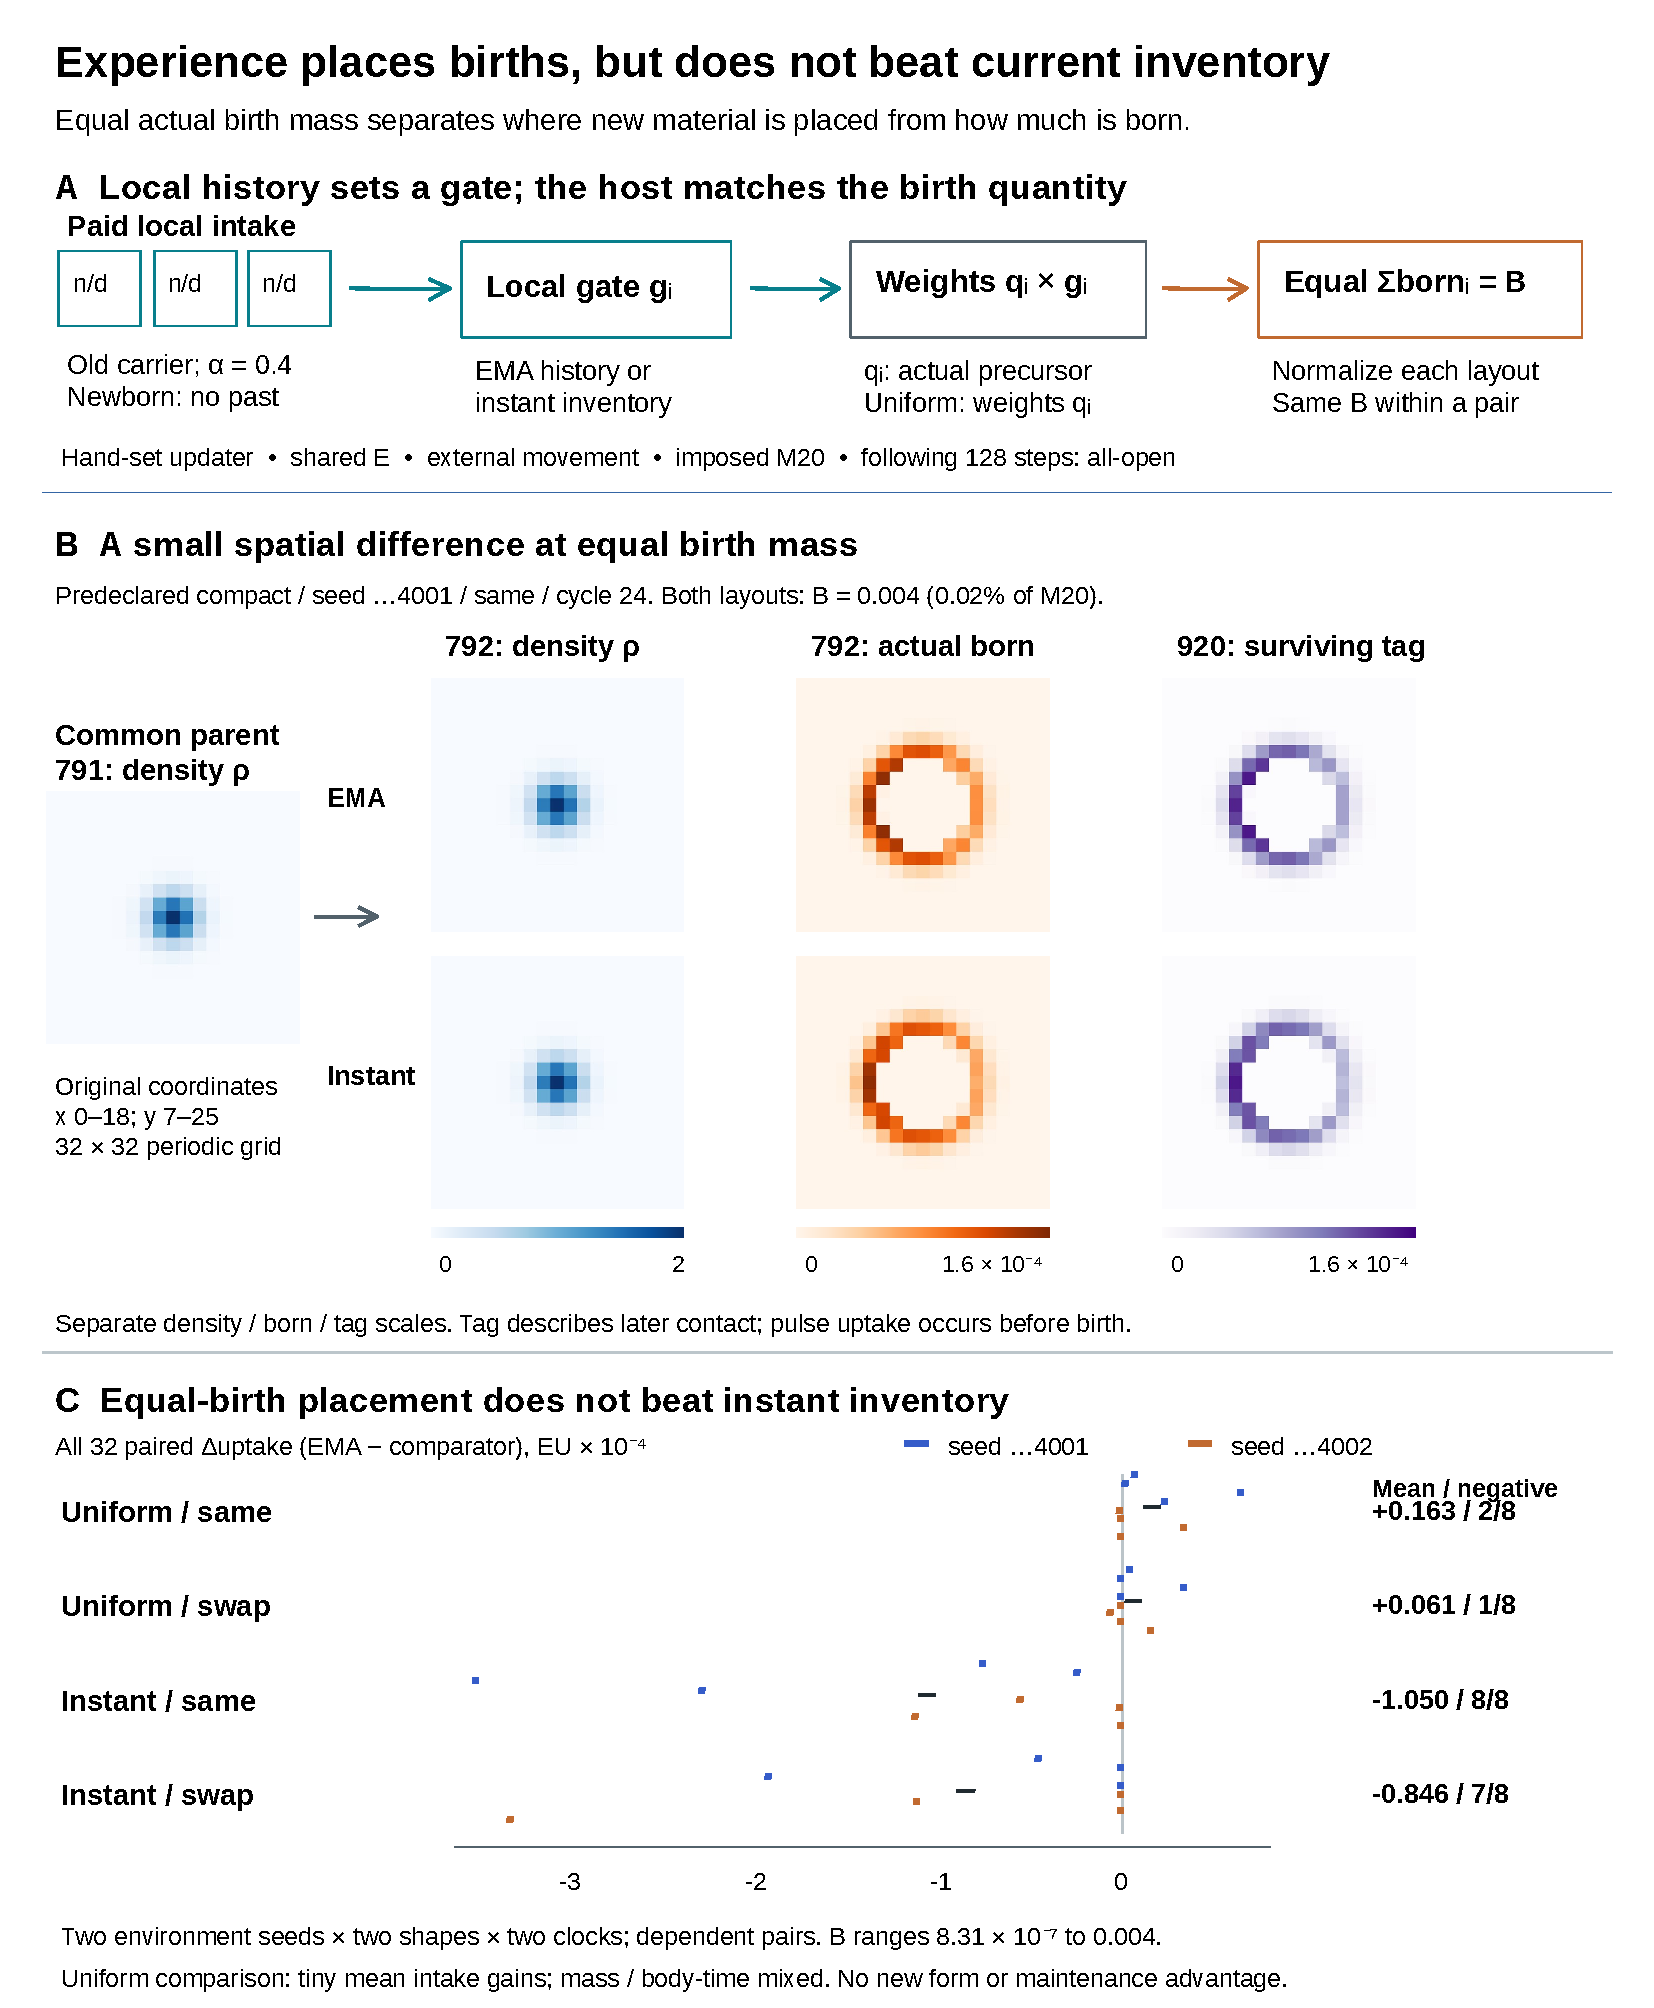
\includegraphics[width=\linewidth,height=0.77\textheight,keepaspectratio]{work/method_renewal/figures/birth_placement/birth_placement.pdf}
\captionsetup{font=footnotesize}
\caption{\textbf{History changes material placement but does not outperform current inventory in matched small births.}
\textbf{A,} Completed local intake supplies a hand-set, material-carried EMA and a birth gate. The host matches total admitted mass $B$ within each history/uniform or history/instantaneous-resource pair; the policy does not observe its returned precursor $q$. Movement, shared energy and the mass cap remain prescribed.
\textbf{B,} Predeclared compact body, seed 202610184001, unchanged ports: saved parent 791, birth 792 and tag 920. Crop fixed in original coordinates; density and material scales differ. Both arms admit $B=0.004$, 0.02\% of the mass cap. Tags start after pulse uptake. For fully paid, nonreproducing tags, uniform turnover fixes total retention, not contact. Tags do not measure energy flow. Recovery shares a requested movement tape and 128 all-open steps.
\textbf{C,} All 32 paired differences in subsequent whole-body uptake, in the displayed $10^{-4}$ units. Colours identify the two environmental seeds; black marks are arithmetic means, not uncertainty intervals. Shapes, pulse times and futures are dependent. History gains slightly over uniform gating of actual precursors, but loses to current inventory in 15 of 16 pairs; mass and body-time effects do not uniformly follow uptake. The intervention does not establish a new morphology or a learned update rule.}
\label{fig:birth-placement}
\end{figure}


The intervention therefore shows that material placement can matter even when its amount is held fixed, but the old carrier's uptake history does not improve on instantaneous resource in these small birth opportunities. Admitted material is at most 0.02\% of pre-pulse mass. Tags follow only that material and apportion later contact, without identifying an energy pathway or a mediator. Their equal total retention is structurally fixed in this fully funded window: uniform turnover gives $T_{128}=B(1-0.0002)^{128}$, irrespective of placement (Methods). Spatial contact and whole-body acquisition can nevertheless differ. Crucially, birth follows the pulse's uptake; this intervention allocates the proceeds of a harvest rather than preparing capacity to affect that harvest. Neither the tiny births nor their subsequent redistribution establish a new stable morphology.

To test an action with an explicitly future return, a separate host requires paid functional preparation eight steps before resource arrival. Capacity is limited by old tissue, transported with survivors and absent from newborns; it changes actual local uptake when mature. The body consists of two prescribed stationary material leaves with a shared energy reserve and mass cap. Two opposite, genuinely paid histories were transplanted as controller contents into the same complete physical state. Under the same current cue and empty inventory, preparation matched to the future obtains approximately 5.70 resource units and gains 2.12 energy units; opposite preparation obtains approximately 0.285 and loses 1.66. The paired energy advantage is 3.776 and 3.774 for the two future directions. This content intervention establishes a useful preparation opportunity, not naturally identical bodily histories or an advantage of a particular update rule.

We then selected an eight-parameter local update rule on two training environments and fixed its parameters before testing four new seeds. Local states continue to update from paid, completed observations. In the twice-changing environment, mean uptake is 146.538 for the selected rule, 149.073 for last-contact memory, 127.562 for a fixed rate-0.5 average and 111.370 for frozen writing. The selected rule loses to last-contact memory on all four seeds in both stable and changing environments. Their recovery delays are identical in all eight seed--change windows. Updating nevertheless matters: relative to the same-prefix frozen branch, the selected rule gains 35.168 uptake units and 77.762 mass--steps of body-time in the changing condition. Relative to last contact, body-time is higher by only 0.074 mass--steps and actual payment lower by 0.200 energy units; relative to the fixed average, uptake is higher but body-time lower by 2.610 mass--steps. Thus the comparison is not a uniform ranking across outcomes.

All 56 test paths survive. The selected rule, last contact, fixed averaging, frozen writing and instantaneous-inventory control finish at approximately the same capped energy, 31.027; higher uptake does not imply a higher final reserve. The instantaneous control falls back to uniform preparation because inventory is empty at commitment. It is therefore a weaker information comparator than recent same-cue feedback. The common exploration floor yields legal feedback on both sides, and local contingencies remain deterministic between changes, making last contact particularly effective. These completed tests support the value of updating preparation after a change, but not extra value from training this update rule. They do not establish the necessity of spatial memory or a general failure of learned local adaptation.

To ask whether uncertain feedback makes evidence accumulation more useful, we next retained the preparation physics and introduced conditionally independent noisy supplies at the two ports. A distinct six-parameter discounted-count updater was trained and frozen before four new environmental seeds were tested. With supply probabilities 0.7/0.3 and hidden-map switching probability 0.04 per cycle, mean uptake is 119.524 for this rule, 120.838 for local last contact, 123.376 for a training-selected count estimator and 124.654 for local Bayesian inference using the known generating parameters. The learned rule exceeds these comparators on only two, two and one of the four seeds, respectively. Relative to Bayes, it also has lower final energy by 0.821, lower body-time by 15.602 mass--steps and higher actual payment by 0.360. Bayes gains 3.816 uptake units over local last on average, but only two worlds improve. This is a descriptive opportunity for accumulation, not a reliable cross-world advantage or an advantage of training the updater. The learned and local-last rules have identical recovery lags in all five realized change windows, including one censored window; Bayes is not uniformly faster.

In a specified negative control, supply probabilities are 0.8/0.2 and the switching probability is 0.25. A single local observation then determines the preferred preparation direction for both Bayes and local last, despite their different confidence values (Methods). The owner's exact comparison finds all 4,096 paired physical scalar steps identical. The learned rule gains 20.913 uptake units and 3.844 final energy units over its same-prefix paid-frozen branch, yet exceeds local last by only 0.782 uptake units while losing 0.291 final energy units and 5.793 mass--steps of body-time. Thus a benefit of continued writing does not establish a better update rule. In the main noisy condition, uniform preparation has lower uptake but greater mean body-time and lower payment than either the learned rule or Bayes. All 56 futures survive. An additional paired-last policy integrates both ports' paid receipts and is kept outside the same-local-information comparison. Each condition has four environmental seeds, not 98 independent observations from its sensed cells. Neither this closed candidate nor the earlier trained rule establishes superiority over the relevant simple controls.

We next allowed paid observations before commitment, while retaining natural uptake feedback for every policy. A fixed local Bayesian estimator processes both channels; only five observation and preparation coefficients are searched. Twelve evaluated proposals do not improve the initial hand-designed policy: its training score remains 49.023479, and its original coefficients are retained. The source arm named \texttt{learned} therefore denotes a selected incumbent, not newly learned behaviour. In four new worlds with informative early sensing, mean uptake is 130.914 for this incumbent, 121.235 when no extra observations are purchased, 132.243 for a fixed uncertainty-threshold rule and 133.607 for a fixed value rule. The incumbent gains uptake over no purchase in all four worlds, at 2.303 additional payment units on average; final energy improves in only one world and body-time in two. Against the value rule, uptake is lower in two worlds and tied within numerical precision in two; against the threshold, it is lower in one and tied in three. Preparation-gain swap controls reproduce their corresponding parent policies because the search retained the original gain. Neither buying useful information nor completing the search establishes an optimized policy advantage.

Continued feedback still matters in this intervention. Relative to paid-frozen content from the same acquired complete state, the incumbent gains 39.030 uptake units, 10.433 final energy units and 38.385 mass--steps of body-time, with all three differences positive in every world. Freezing the observation mask while retaining content updates instead gives a smaller mean uptake difference of 3.264, positive in only two worlds. In the same-price uninformative-sensor condition, the incumbent and value rule buy nothing and match the no-purchase control within numerical precision. Always observing adds 9.542 payment units without increasing uptake. The policies know that this sensor is uninformative; abstention is model-based selectivity, not learned identification of failure. All 88 futures survive. Eight content-frozen recovery windows remain censored, and the fixed value rule recovers at least as quickly as the incumbent in each corresponding window. These results establish an executable paid-observation opportunity, while closing this search candidate without a new observation or preparation ability.

\subsection*{Learning local responses changes spatial action without improving control}
We next tested response learning in a different physical host: two-kernel cellular growth, conservative material transport and local energy, with local directional drive rather than whole-body translation. A material-carried ridge model uses completed eight-step contact and old-material energy changes to predict action responses. Two acquired bodies and two related resource geometries yield four dependent contexts. Five policies continue from each identical acquired body, inventory, environmental cursor, learning state and random state; resource geometry changes after 48 of the 96 continuation steps. The updating and frozen models request identical first actions. Twelve completed-block updates subsequently alter the learned content and the recorded spatial actions, although the bodies have also diverged by then. The experiment therefore establishes an executed response-learning loop, not an isolated causal model of each material element's action.

The decisive comparison is with a recent-return controller using the same delayed feedback and material-transport semantics. Across the four contexts, the response model acquires 6.779 fewer resource units, ends with 7.171 less energy and spends 7.970 more on movement on average; all three contrasts have these signs in every context. Relative to fixed fuel-gradient control, uptake is lower by 115.222 while body-time is higher by 44.603 in the host's time units, preserving a real acquisition--retention trade-off. Relative to frozen content, uptake is lower by 5.910 in every context, with mixed signs for final energy and body-time. Relative to no additional drive, final mass, final energy and body-time are lower in all contexts (mean differences $-11.786$, $-82.629$ and $-38.824$), while movement costs 82.340 more. The no-drive policy retains the host's passive transport and its costs. These comparisons do not support useful control beyond the strong recent-return baseline.

All twenty futures remain alive. Nevertheless, every policy loses mass during the last 32 steps in the porous body and gains mass in the four-lobed body; neither observation establishes a steady state. The model's smaller reported conditional prediction errors are measured on each policy's own trajectories and surviving carriers, not a common forecast test set. Accounting for all registered deaths preserves physical losses but does not remove this selection from local fitting. Thus updated response estimates, changed spatial actions and improved bodily control remain separate claims. This particular local ridge candidate is closed without a claim of predictive or control superiority.

\subsection*{Local records change action, but their value depends on bodily context}
A separate terminal-feedback experiment uses completed direct records and paid, locally delivered messages in a fixed recent-return estimator, without retraining the response model. The original time-gated job completed six porous-body futures but only the four-lobed body's acquired prefix. A separately authorized continuation then restored that exact prefix and completed five four-lobed-body futures without replaying acquisition. The original job remains partial; the registered-old-support Eulerian arm remains unrun for the second body. The following comparisons retain each body's outcomes separately.

In both bodies, updating and frozen-content branches have identical physical scalars and payments for their first 64 steps. At clock 256, all recorded public body, resource, energy, direct-record and message fields still match, while estimator contents differ. The next choices differ at 1,763 sites in the porous body and 1,094 sites in the four-lobed body; the latter involve 424.447 units of current material. Actual requests differ at step 257. Ignoring message content also changes the first choice after acquisition. These checks establish that legally received content enters local action; the sites and material amounts are not independent experimental units.

The bodily consequences have opposite signs (Table~\ref{tab:terminal-bodies}). Updating improves final mass, energy, uptake and body-time over frozen writing in the porous body, but lowers all four in the four-lobed body. Using messages lowers uptake in both bodies; its energy and body-time benefits in the porous body reverse in the second. Against no extra drive, both bodies gain mass and uptake, yet energy and body-time decrease in the porous body and increase in the four-lobed body. Thus the second body provides a positive example of active control over passive continuation, alongside a negative result for this particular update and message-use rule. Compared with full-current-body Eulerian shear, the four-lobed recent-record policy saves 38.432 movement-payment units and gains 2.324 final energy units, but loses mass, uptake and body-time. This comparator also changes execution support and is not a pure information control. All six porous-body futures survive but end below their starting mass; the five second-body futures survive and gain mass and energy over their own common start. Neither finite outcome establishes steady maintenance. The second-body completion followed inspection of the first body's results in one previously used layout, so it is descriptive follow-up, not independent environmental replication or held-out confirmation.

\begin{table}[htbp]
\centering
\small
\begin{tabular}{llrrrr}
\hline
Body & Comparator & $\Delta M$ & $\Delta E$ & $\Delta U$ & $\Delta$ body-time \\
\hline
Porous & Ignore messages & +2.568 & +1.061 & -4.507 & +8.629 \\
Porous & Frozen writing & +7.424 & +3.701 & +3.081 & +7.770 \\
Porous & Full-body Eulerian & +2.931 & +37.048 & +4.719 & -7.065 \\
Porous & No extra drive & +1.041 & -49.997 & +58.531 & -26.515 \\
Four-lobed & Ignore messages & -2.990 & -3.434 & -5.843 & -19.798 \\
Four-lobed & Frozen writing & -12.544 & -2.914 & -4.724 & -18.510 \\
Four-lobed & Full-body Eulerian & -35.165 & +2.324 & -30.035 & -82.923 \\
Four-lobed & No extra drive & +23.987 & +17.851 & +51.136 & +79.851 \\
\hline
\end{tabular}
\caption{Body-specific effects of using recent local records. Each entry is recent-record control minus the named comparator over a 128-step continuation from that body's shared acquired state. $M$ and $E$ are final mass and energy; $U$ and body-time are cumulative over the future. Positive and negative differences are retained without averaging the two bodies. These are dependent comparisons in one known layout, with no uncertainty intervals or claim of independent environmental replication. No extra drive retains passive transport and actual movement costs.}
\label{tab:terminal-bodies}
\end{table}

A follow-up asks whether received records become more useful when their source context is retained. Before each action, the sign of the local fuel-gradient projection onto the shear direction labels three source classes; these labels travel with the registered material. Fixed readers select the currently matching class, reverse its sign, or pool all classes, while direct records retain the same pooled representation. From two newly acquired common parents, matching versus reversed and pooled reading changes the first requested drive at respectively 232 and 115 sites in the porous body, and 115 and 45 sites in the four-lobed body. Complete public, writer and random states match before this first choice. Later choices follow different bodies and are not repeated interventions at an identical state. These site counts establish an action difference, not additional experimental replication.

Matching has conditional bodily value. Relative to pooling, it changes final mass, energy, uptake and body-time by $(+1.879,+1.138,+2.658,+6.426)$ in the four-lobed body, with all four also positive against reversed reading. In the porous body, the corresponding differences are $(+1.182,-2.977,+0.027,-5.085)$: the small mass and uptake gains accompany energy and body-time losses. A fixed fuel-gradient controller nevertheless exceeds matching on all four measures in the four-lobed body. Relative to no extra drive, matching lowers energy by 50.193 and 11.030 and body-time by 55.023 and 17.728 in the porous and four-lobed bodies, respectively, despite greater uptake in both. No extra drive still entails passive transport and actual movement payments. Thus context-sensitive reading can improve on pooled records without establishing control value beyond the strong fixed alternatives.

Selected record exposure and fallback to pooled evidence differ between readers, so this comparison does not isolate semantic matching from the amount and composition of available evidence. Saved initial requests and actual endpoint fields show the spatial intervention and its consequences; the three readers produce closely similar gross body organization, while fixed controls produce more visible differences. This is a limited inspection of saved composites, not a review of every field trajectory or evidence for a new stable morphology. All twelve futures survive the finite window. The two bodies occupy one known rotated layout, and the new acquisitions and packet charge differ from the preceding experiment; cross-experiment differences cannot be assigned to source labels alone.

Completed consumption can also inform resource routing without assigning a return to a moving tissue element. A separate native-host experiment records how much precursor and fuel arriving through each spatial edge is subsequently used, and returns that local description to the sending neighbour. These records alter actual paid pumping, including its direction. The memory belongs to fixed spatial edges rather than travelling with tissue, and proportional attribution within mixed inventory does not identify causal credit. A proposed minimum-of-use score fails its development criterion; the continuation uses a hand-set exponential average, merged with the identical baseline, without a trained update rule. Two known mature parents, two related supply placements and six arms yield 24 complete 160-step futures, all retaining tissue.

The comparison also changes whether pumping occurs. A later read-only audit of the two matched first-decision states finds EMA/demand requested and executed totals of 0.324439/0.201948 and 0.768875/0.489266. Demand has zero directional weight at 9 and 23 sources where EMA pumps. At sources active in both arms, total proposals match to numerical precision while directions still differ. Thus the whole-policy comparison combines execution quantity and direction from the first decision, before the physical trajectories diverge. Static and changed conditions coincide at that decision and do not add independent states.

The routing comparison again separates tissue gains from energetic benefit. Relative to immediate local demand, the consumption average increases mean uptake by 4.505, body-time by 2.648 and surviving new tissue by 1.745, while reducing final energy by 2.334 and adding 3.312 in pumping cost. These signs hold in all four dependent contexts. Relative to inventory-gradient diffusion and a recent-flow estimator, mean final energy falls by 0.532 and 0.239 and uptake by 2.544 and 1.423, respectively, despite lower pumping costs. Stopping writes produces a small mixed contrast: continued updating changes mean energy by $+0.0025$, body-time by $-0.0100$ and uptake by $-0.0677$, with both positive and negative context-specific effects. Actual routing differs, but these outcomes do not establish additional bodily value from the updates. Relative to no additional pump, mean uptake and body-time increase by 13.471 and 6.411 while energy falls by 3.411; that comparator retains native passive processes.

Here surviving new tissue is measured from the mature-parent clock 384 and includes births during acquisition, not only the evaluated future beginning at clock 448. Saved fields show local differences in replacement within broadly similar porous and fuller bodies, rather than a new stable morphology. The four contexts share two known parents and correlated placements, and are not independent environmental replications. Feedback, storage and computation carry no additional charge, although pumping is paid. These finite continuations connect actual consumption to routing while leaving both its incremental control value and longer-term maintenance unestablished.

\subsection*{Newly formed bodies do not establish sustained resource tracking}
The preceding controls use already formed bodies. A separate outer search tests whether new bodies can form and support useful action under a common finite resource schedule. Sixteen new lives, eight in each of two generations, start with gifted mass and energy of 64 each and no extracellular precursor or fuel. Twelve compact, ring and separated-seed candidates die at steps 17--27. All four double-lobe candidates pass the unchanged formation gate, ending at masses 47.124, 47.961, 49.083 and 36.131 after 128 steps, although all still lose mass during the last 64 steps. In this initial search, initialization families are coupled to different rule sources, so that contrast alone does not isolate geometry or a particular gene. The frozen Pareto and identifier rule selects a first-generation parent; the second generation is not uniformly better.

That parent's actual complete state branches once into passive and continuous fuel-gradient control for 256 steps. Gradient control gains 5.597 uptake and 30.348 body-time units, while paying 1.765 more for movement and losing 0.841 final mass and 1.899 final energy relative to passive continuation. It therefore fails the registered joint requirement of greater body-time without lower final energy. Final mass/energy are 21.471/37.894 for passive and 20.630/35.995 for gradient control; both decline in both measures during the last 64 steps. The saved sequence shows the initially perforated double-lobe body becoming a more filled small cluster, failing to keep pace with the moving input region, and shrinking late. The plotted input region marks the last applied fuel supply, not carried inventory or future information. This is one selected-parent comparison under standard mutation and selection, with no local writer or lifetime learning; finite survival does not establish steady maintenance or a new algorithm.

A completed factorial comparison resolves this particular rule--initialization confounding by independently crossing the four frozen base rules, R0--R3, with the four actual initial geometries and two supply placements. At identical gross precursor and fuel input, the static-patch arm is compared with externally supplied input distributed over the body's pre-step neighbourhood. Of 32 dependent combinations, 23 become extinct and nine retain tissue at step 128. R0 and R3 retain none of their eight combinations, whereas R1 retains three and R2 six; every separated-seed initialization fails. R1, which failed from its original ring initialization, retains both compact-initialized bodies and forms a smaller ring-shaped density distribution. R2 supports compact and ring as well as double-lobe starts. Compatibility therefore matters within these frozen rules and initial states; the earlier double-lobe-only outcome was not a geometry-only result.

Supply placement also changes actual tissue replacement. For R1 with compact initialization, neighbourhood-supported rather than patch supply raises final mass from 51.216 to 64.572 and retained new tissue from 0.044 to 15.500, while surviving founder material falls from 51.172 to 49.072. This is more newly generated tissue, not simply greater preservation of the initial gift. R1 with a double-lobe start dies at step 126 under patch supply but retains mass 40.772 under supported supply. R2 with a double-lobe start likewise increases retained new tissue from 2.986 to 16.805. These gains still fail the registered joint extension gate: all nine surviving paths lose tissue over the last 64 steps. Even R1 compact under supported supply produces only 7.396 units against 7.650 units of death in that interval. No combination is extended, and final mass above the initial gift or rising energy does not establish self-maintenance.

The counterexamples delimit this supply effect. R3 with a double-lobe start takes up more under supported supply yet dies three steps earlier, at 112 rather than 115. All recorded tissue death in this comparison occurs in the rule stage, with zero actor injury or starvation death; this accounting location does not establish resource-independent failure of a rule. Both precursor and fuel placement change together, and precursor rejection precedes fuel rejection in the actual birth ledger. Their ordered totals cannot identify an isolated precursor shortage. The intervention supplies resources externally, with no learned controller or lifetime change of rule, and its 32 combinations are not independent environmental repetitions.

A subsequent turnover-oriented outer search finds limited genetic improvement without achieving maintenance. Four fixed rule sources are crossed with compact and double-lobe starts and two static supply layouts, giving sixteen first-generation paths. Only R2 meets the reproduction criterion in all four contexts. The initial implementation excludes ineligible proposal parents instead of filling the second parent slot: only R2's two children are evaluated before selection and continuation. A separate completion subsequently evaluates the two already specified R1 children, filling the four-child formation comparison (Table~\ref{tab:turnover-formation}). The eligibility-first retrospective order is p0c0, p0c1, p1c1, p1c0. The originally selected p0c0 remains first, but this later ranking cannot convert its earlier continuation into a prospective test of the full four-child selection. Seven first-generation extinctions and all unselected offspring remain in the record.

\begin{table}[htbp]
\centering
\small
\setlength{\tabcolsep}{4pt}
\begin{tabular}{llrrrrc}
\toprule
Parent & Child & \multicolumn{2}{c}{Compact} & \multicolumn{2}{c}{Double lobe} & Contexts\\
\cmidrule(lr){3-4}\cmidrule(lr){5-6}
 & & Colocated & Separated & Colocated & Separated & passing\\
\midrule
R2 & p0c0 & 65.073 & 60.165 & 56.350 & 52.035 & 4/4\\
R2 & p0c1 & 56.777 & 53.052 & 50.203 & 46.698 & 4/4\\
R1 & p1c1 & 64.694 & 60.232 & 45.871 & 22.700 & 3/4\\
R1 & p1c0 & 62.229 & 56.335 & 39.160 & 2.923 & 3/4\\
\bottomrule
\end{tabular}
\caption{\textbf{Completed four-child formation coverage at life step 128.} Entries are final mass; each context passes when final and last-64-step mean mass are both at least 32. Eligibility requires all four contexts, so both R1 children remain ineligible. Child labels abbreviate the archived generation-two identifiers. Rows follow the retrospective eligibility-first ordering: the two R2 children were evaluated before the original selection and continuations; the two R1 children were evaluated later. The four geometry--supply contexts are dependent development conditions, not independent environments. Formation eligibility does not establish tissue replacement or step-384 maintenance.}
\label{tab:turnover-formation}
\end{table}

Both added R1 children retain tissue through step 128 and pass in three contexts, but their double-lobe separated-supply masses are only 2.923 and 22.700. All eight added paths have births below deaths during the last 64 steps. At step 128, p1c1 exceeds its direct genetic parent in mass, energy, body-time and retained new tissue in every context. In the separated double lobe, however, its mass gain of 16.126 comprises 14.765 more founder material and only 1.361 more new tissue. The other added child, p1c0, has lower final energy than its parent in all four contexts and mixed changes in the other measures. Saved sequences show compact starts forming small rings and separated double lobes shrinking, with p1c0 reduced to a small patch by step 128. These are fixed-rule comparisons from matched life-zero configurations with different formation histories, not interventions on the same acquired body state.

Against its direct genetic parent with pumping maintained, the selected child increases final mass by 1.398--2.435, final energy by 1.905--5.515 and whole-life body-time by 32.161--50.606 across the four contexts at life step 384. This is finite inherited improvement under fixed within-life rules. It does not uniformly improve replacement: in the double-lobe separated-supply condition, surviving post-birth tissue is lower by 1.265 while founder retention is higher by 2.663. Parent and child have different formation histories. A separate intervention branches the child's identical complete step-128 state into continued pumping and no further pumping for 256 steps. Continued pumping increases mass, body-time and retained post-birth tissue in all four contexts. Energy also increases in both separated-supply cases and the colocated double lobe, but falls by 1.724 in the colocated compact body. The stopped-pump arm retains passive transport and the shared first 128 steps of pumping, and actual continuation costs differ.

All twelve original parent/child continuation paths nevertheless fail the step-384 maintenance criterion. In each of their two final 64-step windows, births remain below deaths; all 24 windows fail both exact and $10^{-8}$-tolerant balance. The selected child's colocated cases still gain energy late while losing mass, whereas its separated-supply cases lose both. Saved sequences show a small hollow ring under R1 and thicker compact bodies under R2 and its offspring; double-lobe starts retain asymmetric lobes under colocated supply and become connected, flatter bodies under separated supply. The parent--child shape differences are limited and do not establish a new morphology class. These four related development contexts support conditional inherited and transport effects, not independent environmental confirmation, lifetime adaptation or steady tissue replacement. The later formation completion adds no step-384 continuation and leaves the original selection-before-coverage chronology unchanged.

A reciprocal rule intervention separates the effects of the current rule package from the acquired state produced during formation. At life step 128, each actual R2-parent and selected-child state either keeps its rule or receives the other's rule and kernels, yielding two histories crossed with two current rules in each of the four contexts. Eight new 128-step switches are compared with eight archived, exactly matched same-rule continuations. On both histories, the current child rule increases mass at step 256, energy and continuation body-time in all eight comparisons: mass gains are 1.933--2.796 and energy gains 1.897--5.366. Conversely, with the current rule fixed, child-history bodies have lower final mass and lower late-64-step body-time in all eight comparisons, with mixed energy differences. The current rule package therefore contributes to the finite benefit; the child formation history alone does not explain it. Between-history differences include inventory, turnover and the rest of the acquired state, and do not isolate geometry or show that history is irrelevant.

The same intervention sharpens the distinction between retaining a body and replacing its tissue. In separated-supply double lobes, switching to the child rule increases final mass by 2.588 on the parent history and 2.442 on the child history. These gains comprise 2.743 and 3.193 more surviving founder material, offset by 0.154 and 0.751 less retained tissue born after life zero. The other six comparisons retain more post-life-zero tissue, but this label includes tissue born before the step-128 switch; the old baselines have no separate post-switch lineage tag. Saved fields show thicker compact rims and connected, shrinking double lobes, without establishing a stable new morphology.

Only the parent-history compact and double-lobe colocated bodies switched to the child rule pass the first 64-step maintenance window. Thus two of 32 windows pass, but none of the sixteen paths passes both successive windows. Births fall below deaths in every late window, with deficits of 0.965--3.482. The external rule replacement has no priced biological rewrite action and supplies no evidence of lifetime learning. These dependent development comparisons establish conditional finite effects of the whole rule package, while preserving the original step-384 maintenance failures and selection chronology.

A resource-conditioned mixture then tests whether training can improve the use of two fixed native growth responses. Its four parameters map local precursor, fuel and energy to a mixing weight. Two rounds of cross-entropy search produce ten nonzero proposals, none eligible for deployment. Eight improve the worst-context retention of newly born tissue but lose mass, energy or body-time elsewhere in the joint criterion. The zero parameter vector is retained, and the best tested constant is the original weight $w_0=0.5442572838640933$. All proposals remain reported, including four extinct training trajectories at constant weights 0 and 0.25. This completed search produces no new trained behaviour and does not establish that the function family is intrinsically incapable of improvement.

After selection is frozen, two new input seeds and two related initial shapes supply four validation contexts. The selected, best-constant, pooled and original-weight roles are exact aliases registered before execution: twenty named roles represent only eight physical futures. A simple pre-state greedy rule, which uses the available growth responses and admission calculation, improves final mass, energy, body-time and actual post-step-128 tissue retention over $w_0$ in all four contexts. Mean gains are 4.371, 3.616, 50.673 and 0.706, respectively, with 1.566 more pumping cost. Most of the mass gain is instead 3.666 more retained material already present at step 128. This label includes both founder material and tissue born during acquisition; it is distinct from the life-zero founder label used above. The selected constant rule therefore fails to beat this simple comparator. Greedy has additional structural-response information and unpriced computation, so the comparison does not isolate the effect of training alone.

Greedy passes only the first 64-step maintenance window in each context. These are the four successes among 32 physical windows; every later window has births below deaths, and none of the eight futures passes the final two windows or all four. All eight retain tissue, but finite survival and the positive final contrasts do not establish sustained replacement. In the saved first-seed examples, greedy retains a fuller compact body and a wider double-lobe bridge, accompanied by spatially varying weights supplied by the hand-written rule. These are not learned morphology changes. Because the pooled candidate also reduces exactly to $w_0$, its alias supplies no general test of local versus pooled information. The result retains a useful simple generation baseline while leaving the training and sustained-replacement objectives unmet.

Coordinating birth requests further separates immediate production from tissue retained later. A fixed one-hop rule redirects requests that cannot be fulfilled locally towards neighbouring template-supported, affordable capacity. This adds generation semantics: a site with negative native growth response can receive a positive request. It transports requests rather than material, uses extra unpriced neighbourhood information and does not learn. Three coordination arms branch from the same four complete step-128 states, with the earlier greedy futures reused exactly as baselines. The two already-seen input seeds and two related shapes constitute dependent mechanism-development contexts.

Full directed coordination increases cumulative births in every context, but also increases deaths and reduces the amount of post-128 tissue remaining at step 384. Mean birth and death differences are $+1.033$ and $+1.886$; retained new tissue, final mass and body-time change by $-1.418$, $-0.853$ and $-5.186$, respectively, all negative in four of four contexts. Final energy instead rises by $1.507$, accompanied by $1.826$ less pumping expenditure and $0.434$ more birth-fuel expenditure. These are whole-path changes, not a pure cost-mediated effect. The label balance assigns $2.451$ more deletion to tissue born after step 128 and $0.566$ less to material already present then. This accounts for the total death difference but does not identify death by tissue age, location or cause.

Matching the amount offered by each source leaves small directed--uniform differences: mean post-128 retention and body-time gains are $0.0178$ and $0.0156$, while mass and energy signs are mixed. Both matched arms still lose mass, body-time and retained new tissue relative to greedy in all four contexts. Matching applies to a common-state conversion; pumping already produces different energy expenditure immediately afterwards. All sixteen futures survive and pass their first 64-step window, but every later window has births below deaths; none passes the final two windows or all four. First-seed saved fields show similar filling compact bodies and concentrating double lobes across arms, without a new morphology family. Increased birth production therefore does not establish sustained tissue replacement, and the fixed coordination rule supplies no evidence of lifetime learning.

A prospective pulse-cohort comparison tests whether the sign of the current generation response predicts where new tissue will persist. From complete ready states at steps 256 and 320, paired single pulses direct equal source-matched amounts towards sites with $h\geq0$ or $h<0$, followed by unchanged greedy generation and pumping. Here $h$ is the instantaneous signed generation response, not a measure of health. The eight pairs combine the same two input seeds, two shapes and two times. Three pairs admit exactly no extra tissue and have undefined retention fractions; exact aliases leave thirteen physical futures for sixteen named roles. Across the five nonzero pairs, initial extra mass ranges from $1.09\times10^{-4}$ to $3.33\times10^{-3}$. Nonnegative-$h$ sites retain more of that cohort in three pairs and less in two at offset 64. Both losing double-lobe pairs initially lead, then reverse at offsets 55 and 38. Offset 64 includes the pulse and corresponds to birth age 63. Thus the response sign does not universally rank subsequent retention, even over this finite interval.

The prospective observer separates extra pulse births, ordinary pulse births, pre-existing tissue and later births through actual transport and actor/rule deletion. All observed extra-cohort losses occur in the rule stage, but this locates loss rather than identifying its cause. Across all eight pairs, the nonnegative-minus-negative target comparison has mean final mass and energy differences of $-8.88\times10^{-5}$ and $-1.95\times10^{-3}$, with a small positive body-time difference of $5.20\times10^{-5}$; individual signs are mixed. A positive conditional retention average therefore does not establish whole-body benefit. Global totals match at the first conversion to $1.42\times10^{-14}$, after which pumping and realized costs diverge. These already-seen, dependent mechanism comparisons neither explain the earlier continuous-coordination effect by causal mediation nor establish maintenance or learning.

\begingroup\clubpenalty=10000
Changing the spatial distribution of rule deletion provides a separate test of tissue retention. A fixed one-hop operation preserves the original total rule deletion computed for each actual state while relocating its targets among eligible neighbours. Two layouts use capacity-proportional (\texttt{mass}) or uniform weights, with matched outgoing amounts per source. From the same four complete step-256 states, both improve final mass, energy, body-time and retained tissue genuinely born after step 256 relative to the original greedy rule in all four contexts. Uniform-layout mean gains are 0.286, 0.721, 1.256 and 0.227, respectively; capacity-weighted gains are 0.236, 0.582, 1.006 and 0.218. Retention of material already present at step 256 increases in two contexts and decreases in two, so the improvements cannot be described solely as preserving old tissue.\par\endgroup

The capacity-weighted layout improves mass, energy and body-time over uniform in both compact bodies but loses all three comparisons in both double lobes; post-256 retention is higher in only one of four contexts. It therefore has no general advantage over the simpler uniform layout. Preserving deletion at each actual state does not constrain cumulative mortality across diverging futures: the native deletion request itself changes with the body. Neither first-conversion energy and births nor subsequent realized fees are required to match. Despite the finite gains, none of the twelve trajectories passes both predefined 64-step maintenance windows, and births remain below deaths in every final window. Only one of 24 individual windows passes the joint gate. The inspected first-seed fields retain similar compact and double-lobe outlines despite altered local deletion. This external, unpriced coordination establishes conditional spatial-layout value under the tested rules, not sustained replacement, a learned controller or a causal explanation of the earlier pulse-cohort reversals.

Starting from life zero reveals a positive maintenance regime and a limit to the deletion-layout intervention. Sixteen 256-step paths cross two new fixed input tapes, four predefined initial geometries and the original greedy rule with or without uniform deletion redistribution. Uniform redistribution improves final mass, energy, body-time and retained post-128 tissue together only in the four compact and double-lobe pairs. It reduces mass and body-time in all four ring and separated-seed pairs. Post-128 retention increases in six pairs and decreases in two; its positive overall mean does not establish a generally beneficial addition to the generator. All sixteen bodies remain above the formation mass threshold at steps 128 and 256, so failing maintenance here is not extinction.

In contrast to the preceding mature-body continuations, both ring paths under each input tape---the original rule and uniform redistribution---pass all four fixed 64-step maintenance windows, including the final two. The result is unchanged at zero tolerance. In these four ring paths, founders decline from 64 to 35.98--36.87, while living tissue born after life zero reaches 35.31--35.69 and tissue actually born after step 128 reaches 21.95--22.07. This is real tissue replacement during finite maintenance, already achieved by the original greedy rule; deletion redistribution is not necessary for it. The other twelve paths fail the final two-window criterion. Saved fields show the preset ring retaining its hole with changing perimeter density, whereas separated seeds remain separate and shrink. The ring is supplied as an initial geometry, not generated from a compact body. These correlated initial-condition comparisons establish a 256-step regime under the stated resource supply, not a steady state, general morphological robustness or lifetime learning.

\begingroup\clubpenalty=10000\widowpenalty=10000
A further history experiment separates bodily carryover from extracellular resource carryover within this fixed generator. Four previously selected step-128 parents (two input seeds, each with ring and separated-seed bodies) receive opposite orders of upward and downward supply, followed by 64 steps of common central input, or central input throughout. At step 256, the two ordered body histories are crossed with their actual extracellular P/F inventories and tested under both supply directions; central-history controls complete forty 128-step futures. A body history here includes density, intracellular energy and inherited physical state, not just geometry. The common central interval is not assumed to erase either bodily or resource history.\par\endgroup

Bodily direction matching is not consistent across seeds. With either P/F donor held fixed, the first ring seed has negative history-by-probe interactions for body-time ($-1.422$ and $-1.469$) and retained post-256 tissue ($-0.022$ and $-0.024$): the opposite last exposure performs better by these contrasts. The second ring seed has positive body-time interactions but negative post-256 interactions. Separated-seed bodies likewise show opposite-direction matching in the first seed and inconsistent joint signs in the second. By contrast, changing P/F history while holding the acquired body fixed gives positive body-time and post-256 interactions in all eight comparisons, but negative final-energy interactions in all eight. These are differences of differences across probe directions, not absolute gains or percentages mediated by extracellular resources.

The comparison with central-history controls answers a different question. Both separated-seed parents meet the joint mass, energy, body-time and strictly positive post-256 criterion in both matched directions. Both ring parents fail it: post-256 retention is lower by 0.124 in the first seed's downward probe and by 0.679 in the second seed's upward probe, despite higher mass, energy and body-time. Ring bodies already have higher mass and energy after either noncentral acquisition history, so their later endpoint advantages cannot all be attributed to adaptive matching. Nevertheless, twenty of twenty ring futures and sixteen of twenty separated-seed futures pass both 64-step maintenance windows, with identical zero-tolerance decisions. The four failures are all separated-seed central-history controls. Thus noncentral experience can improve replacement relative to a central-history control in selected conditions without establishing a consistent directional bodily memory. These forty futures are related mechanism comparisons, not independent environments; the fixed generator, experimental inventory exchange and finite horizon do not establish a trained learner or a steady state.

Fixed simultaneous spatial coverage supplies a useful comparison to ordered exposure. A new history, $H_B$, gives half of each upward and downward input simultaneously for 64 steps before the same 64 central-input steps. It matches the ordered histories' cumulative input at every cell, while changing instantaneous local dose and synchrony. Each acquired body is then tested with the same actual central-history P/F inventory for its parent. Relative to the central-history body under this common inventory, $H_B$ improves body-time, living post-256 tissue, final mass and energy in all four separated-seed conditions. The respective increases are 15.972--18.566, 2.641--3.276, 4.196--5.106 and 9.470--10.944. Founder retention decreases by 1.224--1.379 while tissue born since life zero increases, so the result is not merely preservation of founders. Rings pass the joint criterion in only one of four conditions: the other three lose post-256 tissue despite higher mass, energy and body-time. Neither endpoint averages nor the extra older tissue rescue those failures.

The ordered histories also pass all four separated-seed comparisons and only one ring comparison under the common inventory. Their differences from simultaneous coverage remain nonzero and mixed. Thus fixed coverage is sufficient for a conditional benefit without proving exact equivalence to ordered exposure, identifying a unique mediator or eliminating all history effects. The acquired body retains intracellular energy as well as density and turnover history. Moreover, replacing its own P/F with the common central-history inventory is an active intervention: across eight ring comparisons it increases final energy but reduces mass and post-256 tissue in every case. In separated-seed bodies it increases body-time and energy in all eight comparisons, but post-256 tissue in only five and mass in only one. This substitution is supplied from an unpriced external reservoir, not a closed reciprocal exchange. All 24 new futures pass both maintenance windows; with eight exactly reused central-history futures, 28 of 32 pass; the four failures are the same separated-seed central-history controls. Zero-tolerance decisions agree. These finite, related development comparisons establish neither learned adaptation nor a steady state.

A conditional third growth response extends finite maintenance without establishing an advantage from training. Added to the original two-response greedy generator, this response is used only when its ready-state admission score exceeds both existing alternatives. Two rounds of an outer two-parameter search evaluate eight proposals and a fixed midpoint on ring and separated-seed bodies. Seven of nine candidates qualify, and a nonzero proposal is selected before validation. Unlike the earlier unsuccessful resource-weight search, this search changes the executed generation response: even an identical initial selection mask can produce a different response magnitude. Parameters remain fixed throughout each lifetime. Validation uses the second input seed under central supply, with no extracellular-inventory substitution; the two shapes and previously used seed are related development conditions, not new independent environments.

The selected response improves final mass, energy and late body-time relative to the original generator in both shapes, but improves actual post-256 tissue only in the separated-seed body. Its ring gains 27.914 mass units while losing 0.850 post-256 tissue units; the increase instead includes 28.764 units of additional retention from the step-256 body. The separated-seed body gains 4.753 post-256 units and passes the joint benefit criterion. Against the stronger fixed-midpoint response, however, selection fails that criterion in both shapes. Post-256 retention increases by 0.047 and 1.768 units, respectively, while final mass falls by 0.238 and 0.314, energy by 0.261 and 1.232, and late body-time by 0.859 and 13.974. Training therefore yields a tradeoff rather than an overall improvement; older retained tissue and newly formed tissue are not interchangeable measures of success.

Both conditional responses, selected and midpoint, pass all four fixed 64-step maintenance windows in both shapes, including the final two windows, with identical zero-tolerance decisions. The original generator fails the final-two-window criterion in this protocol. This does not overturn its earlier positive life-zero ring result under a different protocol. Conversely, forcing the midpoint response wherever its neighbourhood is nonzero causes extinction at clocks 173 and 145 for ring and separated-seed bodies. These deaths remain part of the comparison. Conditional response selection thus supports a finite maintenance benefit that unconditional use does not share, but the trained parameters do not outperform the fixed midpoint on joint bodily benefit. Neither finite maintenance through step 384 nor an externally optimized rule establishes lifetime learning or steady persistence.

The midpoint's preservation of older tissue does not imply that its non-birth-enhancing choices obstruct renewal. To test that interpretation, four complete midpoint bodies at step 256 are branched into policies retaining both classes of third-response choice, only the ready-state birth-enhancing class ($G$), only the remaining class ($R$), or neither. Each policy recomputes its own choices as its state evolves. In all fourteen new futures, the recorded $R$ choices reduce hypothetical ready-state deletion; the corresponding new diagnostic fields are unavailable for the two reused reference futures. The four conditions are the two previously used seeds and two shapes under central supply, not independent new environments.

Keeping $G$ alone fails the joint benefit criterion against retaining both classes in all four conditions (Table~\ref{tab:renewal-choice-outcomes}). Ring post-256 retention increases slightly, by 0.302 and 0.163, while mass, energy and body-time fall. In the separated-seed bodies, post-256 retention also falls, by 4.173 and 2.619. Across the four conditions, mass losses range from 12.639 to 27.523 and energy losses from 17.005 to 60.860. Although $G$-only produces more actual births in every condition, it also loses more post-256 tissue to deletion. Thus retaining $R$ alongside $G$ can support both old material and genuine later-born tissue, particularly in the separated-seed bodies. It is not sufficient to classify a current choice by its immediate birth gain to predict future renewal.

Both classes together pass the two fixed 64-step maintenance windows in all four conditions; $G$-only and neither pass none, and $R$-only passes just the first-seed ring. All zero-tolerance decisions agree. The post-256 factorial contrasts, both minus $G$ minus $R$ plus neither, are positive: 0.587, 3.869, 0.599 and 1.927 for first-seed ring/separated and second-seed ring/separated conditions. These are contrasts between evolving policies, whose masks and realized costs diverge (Table~\ref{tab:renewal-choice-costs}), not a mediator fraction or a decomposition into independent physical doses. They support conditional complementarity, without showing a universal replacement policy, a specific resource or template mediator, or lifetime learning. The earlier ring gain dominated by old-tissue retention remains distinct from renewal.

\begin{table}[p]
\centering
\small
\setlength{\tabcolsep}{3.5pt}
\begin{tabular}{llrrrrrc}
\toprule
Condition & Policy & $M$ & $E$ & Body-time & $L_{256}$ & Post-256 & Maint. \\
\midrule
5601 ring & Both & 99.142 & 165.431 & 616.013 & 78.775 & 20.367 & Yes \\
 & $G$ & 86.503 & 148.426 & 559.523 & 65.835 & 20.669 & No \\
 & $R$ & 95.420 & 157.671 & 604.672 & 75.119 & 20.301 & Yes \\
 & Neither & 85.148 & 143.782 & 552.675 & 63.957 & 21.190 & No \\
\midrule
5601 sep. & Both & 84.264 & 143.407 & 503.481 & 61.881 & 22.383 & Yes \\
 & $G$ & 56.741 & 82.546 & 394.898 & 38.532 & 18.210 & No \\
 & $R$ & 55.964 & 78.086 & 377.855 & 36.623 & 19.341 & No \\
 & Neither & 55.102 & 76.653 & 360.764 & 36.064 & 19.037 & No \\
\midrule
5602 ring & Both & 98.102 & 164.215 & 610.510 & 77.089 & 21.013 & Yes \\
 & $G$ & 83.451 & 143.121 & 540.466 & 62.275 & 21.176 & No \\
 & $R$ & 89.201 & 146.663 & 583.045 & 68.501 & 20.700 & No \\
 & Neither & 79.506 & 133.022 & 521.235 & 58.044 & 21.462 & No \\
\midrule
5602 sep. & Both & 85.678 & 147.950 & 518.426 & 64.059 & 21.619 & Yes \\
 & $G$ & 61.543 & 96.014 & 427.408 & 42.543 & 19.000 & No \\
 & $R$ & 68.274 & 109.880 & 436.783 & 48.723 & 19.551 & No \\
 & Neither & 55.830 & 81.323 & 373.530 & 36.971 & 18.859 & No \\
\bottomrule
\end{tabular}
\caption{\textbf{Combined choice classes support finite maintenance.} Absolute outcomes at step 384 from the same complete step-256 parent within each condition. Seed suffixes 5601 and 5602 denote 202610195601 and 202610195602; sep., separated seeds. Both retains $G$ and $R$; the single-class policies retain only the indicated class. Body-time integrates steps 257--384. $L_{256}$ is surviving fork material, whereas post-256 is surviving tissue genuinely born afterwards. Maint. requires both fixed 64-step windows to pass; zero-tolerance decisions agree. The second-seed Both futures are exact read-only references. These sixteen roles are related comparisons, not sixteen independent environments. Values are rounded; full precision is retained in the source tables.}
\label{tab:renewal-choice-outcomes}
\end{table}

\begin{table}[p]
\centering
\small
\setlength{\tabcolsep}{4pt}
\begin{tabular}{llrrrrrr}
\toprule
Condition & Policy & Pump & Motion & Basal & Synthesis & Template & Birth F \\
\midrule
5601 ring & Both & 5.472 & 3.117 & 7.388 & 4.603 & 0.460 & 9.666 \\
 & $G$ & 3.536 & 3.569 & 6.718 & 4.921 & 0.492 & 10.334 \\
 & $R$ & 4.283 & 3.255 & 7.254 & 4.661 & 0.466 & 9.788 \\
 & Neither & 2.873 & 3.857 & 6.637 & 4.971 & 0.497 & 10.440 \\
\midrule
5601 sep. & Both & 0.641 & 2.167 & 6.034 & 4.858 & 0.486 & 10.203 \\
 & $G$ & 0.379 & 4.432 & 4.747 & 5.013 & 0.501 & 10.528 \\
 & $R$ & 1.119 & 4.456 & 4.543 & 4.959 & 0.496 & 10.415 \\
 & Neither & 0.499 & 4.549 & 4.339 & 4.701 & 0.470 & 9.873 \\
\midrule
5602 ring & Both & 6.336 & 3.066 & 7.322 & 4.721 & 0.472 & 9.913 \\
 & $G$ & 3.868 & 3.687 & 6.490 & 5.016 & 0.502 & 10.533 \\
 & $R$ & 3.706 & 3.610 & 6.998 & 4.846 & 0.485 & 10.176 \\
 & Neither & 3.324 & 4.134 & 6.262 & 5.001 & 0.500 & 10.501 \\
\midrule
5602 sep. & Both & 0.774 & 2.343 & 6.214 & 4.742 & 0.474 & 9.957 \\
 & $G$ & 0.397 & 4.553 & 5.137 & 5.096 & 0.510 & 10.701 \\
 & $R$ & 1.000 & 3.020 & 5.245 & 4.664 & 0.466 & 9.795 \\
 & Neither & 0.542 & 4.911 & 4.493 & 4.747 & 0.475 & 9.968 \\
\bottomrule
\end{tabular}
\caption{\textbf{Realized costs differ across the choice policies.} Cumulative quantities over steps 257--384 for every arm in Table~\ref{tab:renewal-choice-outcomes}. Pump, motion and basal columns are actual paid charges; synthesis and template columns report dissipated energy. Birth F is total birth-related fuel expenditure, including newborn energy and the synthesis/template components, so these columns must not be summed as independent charges. All rows retain the original prices. Across the sixteen logical futures, including the two reused references, unpaid basal charges total $2.092992\times10^{-6}$ and unaffordable pump charges $2.367656\times10^{-5}$; these are not rounded to zero in the records. Complete request, rejection, export, death-energy and cohort accounts remain available. Additional policy arithmetic and observation storage are unpriced.}
\label{tab:renewal-choice-costs}
\end{table}


The fate of tissue already born under the restricted policy remains responsive to subsequent rule choices. At step 320, each of the four $G$-only histories and four both-class histories was forked into both-class or $G$-only continuation to step 384. We registered $C$, material born during steps 257--320 and still alive at 320, separately from older material $O$ and material $N$ born during the subsequent window. Restoring both classes after a $G$ history improves $C$ survival in all four matched comparisons (Table~\ref{tab:postbirth-crossover}). In the two separated-seed bodies, retention rises from 0.6989 to 0.9996 and from 0.7267 to 0.9859, with 2.045 and 1.587 additional units of living $N$. Mass, energy and body-time also improve. The two rings retain more $C$ but less $N$, by 0.215 and 0.139 units. Thus only the two separated-seed bodies pass the joint renewal criterion; better survival of registered tissue alone does not establish improved renewal.

Withdrawing the preservation choices from both-class histories likewise reduces $C$ retention in all four comparisons. However, retaining both classes benefits the survival fraction of older $O$ even more, and produces less living $N$ in all four cases; none passes the joint renewal criterion. A greater survival-fraction benefit for $C$ than for $O$ occurs only in the two $G$-history separated-seed bodies. Support is therefore not generally specific to recently born tissue. The history-by-future-policy interaction in $C$ survival is positive in rings (0.001795 and 0.040158), but negative in separated-seed bodies ($-0.272828$ and $-0.232849$). These interactions compare complete acquired states, including energy, inventories and turnover history, and do not isolate geometry, birth location or a mediator fraction.

All eight both-class futures pass the single fixed maintenance window at steps 321--384; none of the eight $G$-only futures does. This does not extend the earlier two-window result to the crossover paths. Actual charges also differ: after $G$ histories, restoring both classes increases pump payment in rings by 0.868 and 0.916 units but slightly decreases it in separated-seed bodies, by 0.084 and 0.006. Death decreases in all eight comparisons, whereas actual birth decreases in six. These finite observations show that already surviving new tissue can benefit from later policy choices, without demonstrating universal renewal, a newborn-specific mechanism, steady persistence or learning.

\begin{table}[!htbp]
\centering
\small
\setlength{\tabcolsep}{3pt}
\begin{tabular}{llrrrrrrc}
\toprule
Condition & History & $\Delta C$ (pp) & $\Delta(C-O)$ (pp) & $\Delta N$ & $\Delta M$ & $\Delta E$ & $\Delta T$ & Joint \\
\midrule
5601 ring & Both & +2.960 & -9.356 & -0.055 & +10.785 & +12.368 & +25.281 & No \\
5601 ring & $G$ & +2.781 & -1.307 & -0.215 & +3.211 & +7.087 & +5.729 & No \\
5601 separated & Both & +2.789 & -10.479 & -0.842 & +8.383 & +17.198 & +18.068 & No \\
5601 separated & $G$ & +30.072 & +9.905 & +2.045 & +15.431 & +33.893 & +27.660 & Yes \\
5602 ring & Both & +8.789 & -11.154 & -0.024 & +17.726 & +26.688 & +36.455 & No \\
5602 ring & $G$ & +4.773 & -0.372 & -0.139 & +4.121 & +8.909 & +7.705 & No \\
5602 separated & Both & +2.631 & -10.625 & -1.459 & +8.045 & +16.858 & +16.529 & No \\
5602 separated & $G$ & +25.916 & +6.407 & +1.587 & +15.257 & +32.214 & +28.387 & Yes \\
\bottomrule
\end{tabular}
\caption{\textbf{Postbirth support and subsequent renewal separate in matched continuations.} All eight effects are future both minus future $G$ from one complete step-320 parent; conditions share two previously used seeds and two preset shapes. $C$ is material born during 257--320 and surviving to registration, $O$ is surviving step-256 material, and $N$ is living material born during 321--384. Survival-fraction differences use fixed, cohort-specific denominators; pp denotes percentage points. $\Delta(C-O)$ subtracts the $O$ survival-fraction effect from the $C$ effect. $T$ is total body-time during 321--384. Joint success additionally requires noninferior $N,M,E,T$ and the single-window maintenance guards. All zero-tolerance decisions agree. Greater $C$ survival occurs in every pair, but joint success is restricted to the two $G$-history separated-seed bodies. These dependent contrasts do not establish newborn-specific support or steady replacement.}
\label{tab:postbirth-crossover}
\end{table}


Lower final $N$ need not imply poorer retention after birth. Offline reconstruction of the same sixteen futures separates actual births by clock and compares their retention at ages 1, 4, 8, 16 and 32. With equal weights across common birth clocks, or common weights proportional to the mean birth mass in the two arms, the both-class policy has higher retention in 39 of 40 parent-state--age summaries. The exception is the second-seed ring after $G$ history at age 1: differences are $-0.007831$ and $-0.007717$ percentage points under the two weightings. The 2,072 individual clock--age contrasts include 293 negative values, so the aggregate pattern is not universal (Table~\ref{tab:birth-clock-accounting}). Common support shrinks from 63 clocks at age 1 to 32 at age 32; later births are right-censored, not assigned zero survival. These are repeated readings of related trajectories, not additional independent experiments.

A symmetric identity separates the final $N$ difference into birth-amount and retention terms for each birth clock. The summed retention term is positive in all eight pairs. In six pairs, including all four rings, a larger negative birth-amount term leaves less living $N$ at step 384. Both terms are positive only in the two $G$-history separated-seed bodies. Thus the ring endpoint deficit coexists with mostly better age-matched retention; it is not evidence of generally worse postbirth survival. This is exact accounting across births in different evolving bodies, not causal mediation or a comparison of identical material.

\begin{table}[!htbp]
\centering
\small
\setlength{\tabcolsep}{3pt}
\begin{tabular}{llrrrrrr}
\toprule
Condition & History & $\Delta r_1$ & $\Delta r_{32}$ & Negative & Birth term & Retention & $\Delta N$ \\
 & & (pp) & (pp) & clocks/ages & (mass) & (mass) & (mass) \\
\midrule
5601 ring & $B$ & $+0.12144$ & $+3.80726$ & 0/259 & $-0.414218$ & $+0.359377$ & $-0.054841$ \\
5601 ring & $G$ & $+0.03965$ & $+1.48094$ & 48/259 & $-0.423127$ & $+0.208344$ & $-0.214783$ \\
5601 separated & $B$ & $+0.09083$ & $+2.86386$ & 46/259 & $-1.154551$ & $+0.312554$ & $-0.841997$ \\
5601 separated & $G$ & $+0.24018$ & $+14.77341$ & 0/259 & $+0.351651$ & $+1.692984$ & $+2.044635$ \\
5602 ring & $B$ & $+0.10319$ & $+4.23219$ & 0/259 & $-0.540430$ & $+0.516690$ & $-0.023740$ \\
5602 ring & $G$ & $-0.00783$ & $+1.08630$ & 104/259 & $-0.347201$ & $+0.207835$ & $-0.139366$ \\
5602 separated & $B$ & $+0.03440$ & $+0.97787$ & 95/259 & $-1.650496$ & $+0.191305$ & $-1.459191$ \\
5602 separated & $G$ & $+0.25943$ & $+14.57460$ & 0/259 & $+0.016191$ & $+1.570837$ & $+1.587028$ \\
\bottomrule
\end{tabular}
\caption{\textbf{Birth-clock accounting distinguishes endpoint tissue from retention.} All contrasts are future both ($B$) minus future $G$ from the same step-320 parent. Histories are denoted $B$ or $G$. Age-specific rate differences use equal weights across common birth clocks; pp denotes percentage points. The displayed boundary ages bracket the primary set 1, 4, 8, 16 and 32; all five ages and both common weighting schemes are available in the source table. The negative count includes every primary clock--age contrast, with 259 dependent readings per parent and 293 negative readings overall. Common support is 63/60/56/48/32 clocks; right-censored mass is reported separately. Both weighting schemes give the same 39 positive summaries and the same age-1 ring exception. The endpoint birth and retention terms sum to $\Delta N$ before rounding. All eight retention terms are positive, but six negative birth terms outweigh them. These terms are an arithmetic identity across different born material, not causal mediation. Original whole-body, cost and joint-renewal results remain those of Table~\ref{tab:postbirth-crossover}.}
\label{tab:birth-clock-accounting}
\end{table}


A conversion-time test asks whether additional affordable births can improve renewal while preserving the original both-class deletion choice on the current state. At each actual conversion, the branch compares at each site the positive birth requests of the locked both-class response and responses $A,B,C$, retaining a candidate only if its pure admission calculation yields strictly more birth. Deletion, death-released energy and the template remain those of the original both-class choice; only the selected positive request enters the single real admission. This combines later access to the physical state with separation of positive and negative response branches, rather than a learned policy. Six of eight same-parent comparisons activate the change; the two separated-seed both-history comparisons are exact zero effects (Table~\ref{tab:conversion-birth-branch}). The sum of instantaneous shadow gains is distinct from the difference in actual cumulative births: both $G$-history rings have positive shadow gains but fewer actual births and less living $C$ and $N$ at step 384.

Only the seed-5601 separated-seed body with $G$ history passes the full noninferiority and strict-new-tissue criterion, at both zero and $10^{-8}$ tolerances. Its additional living $N$ is 0.00093501 and its energy gain is 0.006051; these are small conditional benefits. Both both-history rings retain more $N$ but less energy, while the seed-5602 $G$-history separated body gains $N$ and energy at the expense of $C$ survival and $C$ body-time. The two zero effects cannot satisfy the strict $N$ increase. All eight candidate futures pass the single 64-step maintenance window, which neither establishes superiority to their references nor extends the earlier two-window protocol. Pump payments already differ, increasing by 0.145490 and 0.104909 in the two both-history rings; extra arithmetic is unpriced. These comparisons do not support general deployment benefit from this birth branch, while retaining its one conditional positive. Neither the local shadow gain, cumulative birth difference nor endpoint $N$ difference is a mediator fraction.

\begin{table}[!htbp]
\centering
\footnotesize
\setlength{\tabcolsep}{3pt}
\begin{tabular}{llrrrrrrc}
\toprule
Condition & History & Shadow & $\Delta$born & $\Delta C$ & $\Delta T_C$ & $\Delta N$ & $\Delta E$ & Joint \\
\midrule
5601 ring & $B$ & $+26.2527$ & $+0.7994$ & $+0.1545$ & $-0.0697$ & $+1.0386$ & $-48.4908$ & No \\
5601 ring & $G$ & $+52.9084$ & $-2.1205$ & $-0.1231$ & $-0.3622$ & $-0.4822$ & $+3.2946$ & No \\
5601 separated & $B$ & $0$ & $0$ & $0$ & $0$ & $0$ & $0$ & No \\
5601 separated & $G$ & $+89.0581$ & $+0.9329$ & $+0.0114$ & $+0.0346$ & $+0.9350$ & $+6.0510$ & Yes \\
5602 ring & $B$ & $+29.6483$ & $+2.4014$ & $+0.0258$ & $+0.0461$ & $+2.6033$ & $-36.2376$ & No \\
5602 ring & $G$ & $+16.7051$ & $-0.3245$ & $-0.0032$ & $-0.0274$ & $-0.2940$ & $+11.3189$ & No \\
5602 separated & $B$ & $0$ & $0$ & $0$ & $0$ & $0$ & $0$ & No \\
5602 separated & $G$ & $+46.9159$ & $+0.6333$ & $-0.0911$ & $-0.0164$ & $+0.4751$ & $+28.1965$ & No \\
\bottomrule
\end{tabular}
\caption{\textbf{More affordable birth requests do not generally improve bodily renewal.} Every numerical entry is multiplied by $10^3$ for readability; mass, energy and body-time retain their own units. Histories $B$ and $G$ denote both-class and restricted acquisition histories; both reference futures use the both-class policy. Shadow is the sum of same-state pure-admission birth gains, whereas all $\Delta$ columns compare actual candidate and reference futures from the same step-320 parent. $C$ is the registered mixed-age cohort, $T_C$ its future body-time, and $N$ actual new material born during steps 321--384. Joint requires noninferior $C,T_C$, final mass, energy and whole-body time, strictly greater $N$, minimum mass 32, and maintenance over the one fixed window. Both tolerances give the same single pass. All eight pairs, including the two zero effects, are shown. Full whole-body outcomes, costs, unpaid amounts and individual guards remain in the source tables. These related development comparisons are not independent environments.}
\label{tab:conversion-birth-branch}
\end{table}


Changing the order of averaging and nonlinear response provides a further test of useful renewal. The fixed third response normally transforms the mean of the two neighbourhood inputs; the alternative averages their separately transformed values, using the same third-response parameters for both. The ordinary ready-state both-class choice and subsequent signed native response remain in place, without training or the conversion-time positive-branch intervention. From four complete step-256 parents, the alternative produces more living post-256 tissue in every 128-step comparison, but less of the existing post-128 tissue registered at 256 (Table~\ref{tab:response-pooling}). Here $O=L_{128}$, $C$ is material born during 129--256 that survives to 256, and $N$ is actual birth after 256; these cohorts must not be pooled with the step-320 registration above. Both rings gain $N$ and mass but lose final $C$ and late-window $C$ body-time; seed 5601 also loses energy. The two separated-seed bodies lose 12.668 and 9.779 mass units and 28.504 and 22.193 energy units, despite their greater endpoint $N$.

None of the four comparisons passes the joint criterion at either tolerance. Both rings pass both fixed maintenance windows, whereas both separated-seed bodies fail the first window because births do not cover deaths; their second windows pass. Lower pump payment in all four comparisons coexists with higher synthesis and template charges. In separated bodies, lower basal payment accompanies reduced body-time while movement payment increases. Thus neither greater endpoint $N$ nor a lower selected charge establishes useful renewal. The fixed both-class reference remains necessary, and this response-order change does not support default deployment. It changes response amplitude, choice and subsequent turnover together, rather than identifying a single spatial-consistency mechanism or the cause of an earlier result.

\begin{table}[!htbp]
\centering
\footnotesize
\setlength{\tabcolsep}{3pt}
\begin{tabular}{lrrrrr}
\toprule
Condition & $\Delta C_{384}$ & $\Delta T_C^{\rm early}$ & $\Delta T_C^{\rm late}$ & $\Delta N_{384}$ & $\Delta T_N^{\rm late}$ \\
\midrule
5601 ring & $-0.1232$ & $+0.4487$ & $-0.0563$ & $+0.5328$ & $+1.3444$ \\
5601 separated & $-5.6019$ & $-8.4626$ & $-15.8664$ & $+0.1712$ & $-0.2118$ \\
5602 ring & $-0.1407$ & $+0.1558$ & $-0.4354$ & $+0.4537$ & $+0.9659$ \\
5602 separated & $-4.4220$ & $-7.1595$ & $-12.4853$ & $+1.2245$ & $+2.0951$ \\
\bottomrule
\end{tabular}
\par\medskip
\begin{tabular}{lrrrrrrrc}
\toprule
Condition & $\Delta M$ & $\Delta E$ & $\Delta T$ & Pump & Synthesis & Template & Movement & Windows \\
\midrule
5601 ring & $+0.1654$ & $-0.0591$ & $+2.7821$ & $-0.1081$ & $+0.1295$ & $+0.0130$ & $+0.0763$ & P/P \\
5601 separated & $-12.6680$ & $-28.5038$ & $-54.9158$ & $-0.3228$ & $+0.1234$ & $+0.0123$ & $+2.3555$ & F/P \\
5602 ring & $+0.1984$ & $+0.4306$ & $+0.7756$ & $-0.9546$ & $+0.0795$ & $+0.0079$ & $+0.1128$ & P/P \\
5602 separated & $-9.7788$ & $-22.1930$ & $-45.6399$ & $-0.3019$ & $+0.2818$ & $+0.0282$ & $+2.0789$ & F/P \\
\bottomrule
\end{tabular}
\caption{\textbf{Averaging after response raises endpoint new tissue while losing existing tissue.} All differences are the average-of-responses alternative minus the fixed both-class reference. The early and late windows are steps 257--320 and 321--384; $T$ is full 128-step body-time and $T_C,T_N$ are cohort body-times. At registration $O=L_{128}$, $C=\mathrm{post128}(256)$ and $N=0$; only actual subsequent birth enters $N$. These labels differ from the earlier step-320 cohorts. Cost columns are differences in actual pump and movement payments and synthesis/template energy charges, not total costs or equal-cost controls. P/F records maintenance pass/fail in the two fixed windows; both tolerances agree. All four joint-benefit tests fail, including the two rings that pass maintenance. Complete costs, small unpaid amounts, rejection fields and all old reference windows remain in the source tables. The four parents are related development conditions.}
\label{tab:response-pooling}
\end{table}


A separate offline test asks whether recent local history improves prediction of tissue retention once current state is known. At 84 prespecified birth clocks from twenty saved trajectories, we reconstructed the fraction of each positive birth source remaining sixteen steps later. Five fixed predictors were fitted once using the four seed-5601 both-class futures, then evaluated on the four seed-5602 both-class futures. Adding two summaries of the previous four local density values reduces equal-trajectory mean squared error by 10.57\% relative to a quadratic current-state model and by 9.56\% relative to a current-state model with the same number of design columns (Table~\ref{tab:history-retention-forecast}). Nevertheless, the prespecified criterion fails: the seed-5602 separated body acquired under $G$ has greater error than both current-state controls and the shuffled-history control. Only three of four trajectories improve. These results retain an average predictive benefit without establishing the required history increment across all four trajectories.

Transfer tests are evaluated separately. The history model improves on both current-state controls in six of eight $G$-only futures, but worsens in both separated bodies acquired under the both-class policy. Moreover, its mean squared error in this transfer group is 0.011970, greater than the constant training-mean predictor's 0.008223. All four response-pooling futures improve relative to the two current-state controls. Neither transfer result rescues the failed primary criterion. The history variables are Eulerian density changes at a fixed location, and current features are observed after conversion but before pumping. They are neither transported memories nor necessarily available before birth. This analysis adds no physical futures or evidence of action value: the earlier $C/O/N$, energy, body-time and maintenance outcomes remain unchanged.

\begin{table}[p]
\centering\small
\setlength{\tabcolsep}{4pt}
\begin{tabular}{lrrrrr}
\toprule
Condition / acquired policy & Mean & Current & Capacity & History & Shuffled \\
\midrule
\multicolumn{6}{l}{\textit{Primary analysis holdout: seed 5602, both-class future}} \\
5602 ring / $G$ & 46.2490 & 18.6381 & 18.3650 & 17.5149 & 18.4734 \\
5602 ring / both & 28.5291 & 13.7608 & 13.7655 & 11.8449 & 13.5480 \\
5602 separated / $G$ & 3.6700 & 1.7366 & 1.7777 & 1.7969 & 1.7727 \\
5602 separated / both & 30.3140 & 20.1287 & 19.7525 & 17.3723 & 20.3516 \\
Equal-trajectory mean & 27.1905 & 13.5661 & 13.4152 & 12.1323 & 13.5364 \\
\midrule
\multicolumn{6}{l}{\textit{Transfer: G-only future, both seeds}} \\
5601 ring / $G$ & 74.6585 & 104.0697 & 104.4891 & 100.5207 & 105.1593 \\
5601 ring / both & 95.5098 & 117.3715 & 117.2502 & 115.7981 & 117.6790 \\
5601 separated / $G$ & 132.1975 & 151.8483 & 151.6422 & 132.8452 & 152.5906 \\
5601 separated / both & 54.6151 & 65.0242 & 64.9562 & 65.6758 & 65.0060 \\
5602 ring / $G$ & 55.0105 & 113.8719 & 112.8804 & 108.5712 & 113.6523 \\
5602 ring / both & 68.3274 & 228.6207 & 229.2723 & 224.2026 & 231.8518 \\
5602 separated / $G$ & 148.0354 & 170.0280 & 169.9242 & 155.9375 & 170.1486 \\
5602 separated / both & 29.4618 & 52.4191 & 52.3939 & 54.0537 & 52.3313 \\
Equal-trajectory mean & 82.2270 & 125.4067 & 125.3510 & 119.7006 & 126.0524 \\
\midrule
\multicolumn{6}{l}{\textit{Transfer: response-pooling future, both seeds}} \\
5601 ring / both & 18.0012 & 8.0513 & 8.1413 & 7.3488 & 7.9888 \\
5601 separated / both & 3.5618 & 15.4950 & 15.2567 & 14.3955 & 15.5046 \\
5602 ring / both & 15.4281 & 9.9644 & 10.0928 & 8.8029 & 9.8555 \\
5602 separated / both & 3.9085 & 6.9933 & 6.8448 & 5.7467 & 6.9392 \\
Equal-trajectory mean & 10.2249 & 10.1260 & 10.0839 & 9.0735 & 10.0720 \\
\bottomrule
\end{tabular}
\caption{\textbf{Recent density history improves average retention prediction but fails the primary criterion.} Entries are mean squared errors multiplied by $10^4$; lower is better. Each trajectory averages birth-mass-weighted errors over its fixed anchors. Mean denotes the constant training-mean predictor; Current is the quadratic current-state model, Capacity adds two current-state cubic columns, History adds two local four-step density summaries, and Shuffled shifts those summaries within each anchor. The seed-5602 separated body acquired under $G$ worsens against both current-state controls and shuffled history. Transfer groups are kept separate: both both-history separated bodies worsen under $G$-only continuation, whose group mean also exceeds the constant predictor. These related trajectories and overlapping anchors do not constitute independent environments or cell-level replicates.}
\label{tab:history-retention-forecast}
\end{table}


Greater total retention under the combined policy does not imply that every material source benefits. An offline paired analysis follows the same material present at each of the eight step-320 parents through the two previously executed futures. Both-class continuation retains more total $O$ and more total $C$ at both 16 and 64 steps, yet every parent--horizon comparison contains occupied sources retained better under $G$-only continuation. At 64 steps, sources with a retention-fraction difference below $-10^{-8}$ account for 21.88--38.04\% of initial body mass (Table~\ref{tab:paired-material-fate}). Their negative contributions range from $-3.287$ to $-0.715$ mass units, even as the net gain in retained pre-existing material is 3.426--17.750. The sourcewise-dominance criterion fails in all sixteen comparisons at both zero and $10^{-8}$ tolerances; the negative mass fractions themselves need not agree across those tolerances.

Differences between the aggregate retention rates of $C$ and $O$ obey an exact identity involving their initial source weights and the same policy-conditioned survival field. They therefore do not identify age-specific support. The 16- and 64-step horizons measure time since the common step-320 state, not birth age; $C$ remains a mixed-age surviving cohort. A separate algebraic calculation for an artificially equiprobable, hidden future-policy label gives a per-source squared-error floor of $\delta^2/4$ (Methods). This is not a bound on the preceding 84 birth-anchor prediction errors or an explanation of their transfer failure. The original bodily outcomes remain decisive: both-class continuation has less living future-born $N$ in six of eight comparisons, and only the two $G$-history separated bodies pass the original useful-renewal criterion. Complete costs, underpayments and the ring counterexamples remain in the paired records. These source maps describe heterogeneous effects of whole future policies, not the effects of switching policy at individual sites.

\begin{table}[htbp]
\centering\small
\setlength{\tabcolsep}{4pt}
\begin{tabular}{lrrrrr}
\toprule
Parent / history & $f^-_{16}$ (\%) & $f^-_{64}$ (\%) & $D^-_{64}$ & $\Delta(O+C)_{384}$ & $\Delta N_{384}$ \\
\midrule
5601 ring / $G$ & 29.3555 & 31.1745 & -1.7672 & 3.4257 & -0.2148 \\
5601 ring / both & 8.1893 & 21.8792 & -0.7151 & 10.8402 & -0.0548 \\
5601 separated / $G$ & 12.3639 & 25.4627 & -1.5790 & 13.3868 & 2.0446 \\
5601 separated / both & 28.9362 & 30.0022 & -3.2875 & 9.2245 & -0.8420 \\
5602 ring / $G$ & 34.4579 & 38.0410 & -1.6271 & 4.2603 & -0.1394 \\
5602 ring / both & 18.6863 & 23.0691 & -2.9820 & 17.7497 & -0.0237 \\
5602 separated / $G$ & 10.6154 & 24.1276 & -1.6791 & 13.6702 & 1.5870 \\
5602 separated / both & 28.6967 & 31.2816 & -2.4856 & 9.5038 & -1.4592 \\
\bottomrule
\end{tabular}
\caption{\textbf{Total preservation gains coexist with sources that favour the restricted policy.} Contrasts are both-class minus $G$-only continuation of the same complete step-320 parent. $f^-_H$ is the percentage of initial body mass at sources whose survival-fraction contrast is below $-10^{-8}$ after $H$ steps. $D^-_{64}$ is their negative contribution to retained pre-existing mass, while $\Delta(O+C)_{384}$ includes all source contributions. Positive total retention does not erase these negative sources. Horizons are elapsed time from 320, not birth age. $N$ is separately born during 321--384 and is not common initial material across arms; six of eight $N$ contrasts remain negative. Dominance also fails at zero tolerance, whose source fractions are retained separately. The original energy, body-time, cost and useful-renewal comparisons remain unchanged.}
\label{tab:paired-material-fate}
\end{table}


Transporting a current generation choice with material provides a distinct executable test, without using the retrospective survival maps. At each ready state, the fixed-midpoint both-class policy chooses weights for responses $A,B,C$. The alternative carries the three density-weighted choice components through that step's single actual transport operator $K$, then applies their receiving-site convex mixture to the original local responses. Each step regenerates and discards these components; they neither accumulate experience nor write memory. From the same eight complete step-320 parents, all eight candidate futures satisfy the single 64-step maintenance criterion, but none passes the complete useful-renewal criterion relative to fixed both, at either zero or $10^{-8}$ tolerance (Table~\ref{tab:material-carried-choice}). Endpoint $C$ decreases in seven comparisons and $N$ increases in only three. All four separated bodies lose endpoint $O,C,N,M$ and $E$; the small body-time gain for the seed-5602 separated body acquired under $G$ does not remove those losses.

The ring comparisons retain the trade-offs. In the seed-5601 $G$-history ring, carrying the choice gains $N=0.075559$, mass $0.136486$, energy $0.067700$ and body-time $0.303109$, but loses $C=0.002704$. In the seed-5602 both-history ring, all three endpoint cohorts increase, while energy, total body-time and $N$ body-time decrease. The saved density and cohort sequences at steps 320, 352 and 384 retain the original ring and four-clump forms with similar macroscopic appearance across policies; the small differences require the quantitative records. These outcomes retain fixed both as a strong comparator and do not support general deployment of this construction. Material association and convex response mixing change together, so this test does not isolate a reference-frame effect. Original physical charges remain, whereas the extra choice-channel arithmetic and transport are not physically priced.

\begin{table}[htbp]
\centering\footnotesize
\setlength{\tabcolsep}{3pt}
\begin{tabular}{lrrrrrrr}
\toprule
Parent / history & $\Delta O$ & $\Delta C$ & $\Delta N$ & $\Delta M$ & $\Delta E$ & $\Delta T$ & $\Delta F_{\rm pump}$ \\
\midrule
5601 ring / $G$ & 63.6304 & -2.7040 & 75.5595 & 136.4859 & 67.6998 & 303.1093 & 68.9002 \\
5601 ring / both & -0.0419 & -0.0307 & 0.8125 & 0.7399 & 6.3698 & 1.3795 & 47.2933 \\
5601 sep. / $G$ & -0.1271 & -0.0400 & -0.0438 & -0.2110 & -1.5676 & -0.7613 & 1.5781 \\
5601 sep. / both & -11.4589 & -5.4794 & -6.8904 & -23.8286 & -47.6368 & -38.8773 & -0.5172 \\
5602 ring / $G$ & 61.1577 & -7.9196 & -13.4270 & 39.8111 & 23.4189 & 23.6122 & -15.5505 \\
5602 ring / both & 0.1888 & 0.0600 & 2.8429 & 3.0917 & -30.4434 & -0.0383 & 24.0255 \\
5602 sep. / $G$ & -20.4487 & -0.1005 & -0.1468 & -20.6960 & -19.1285 & 56.7674 & 0.0064 \\
5602 sep. / both & -10.2885 & -8.3969 & -24.9056 & -43.5910 & -60.7861 & -67.7618 & -4.3878 \\
\bottomrule
\end{tabular}
\caption{\textbf{Carrying current choices with material fails the complete renewal comparison.} All entries are carried-choice minus fixed-both contrasts multiplied by $10^3$ to retain small signs; divide by 1,000 for physical values. $O=L_{256}$ at step 320, $C$ is post-256 material alive at 320, and $N$ is actual birth during 321--384. Cohort, mass and energy entries are endpoints; $T$ is total body-time and $F_{\rm pump}$ cumulative paid pump energy over the 64 steps. Complete physical fees and underpayments remain in the source tables; additional choice-channel computation and transport are unpriced. All eight single-window maintenance tests pass, but all eight complete useful-renewal comparisons fail at both tolerances. Ring and separated-body counterexamples are retained individually, without treating these related parents as independent environments.}
\label{tab:material-carried-choice}
\end{table}


Earlier cue-content tests show six recoveries and three deaths after reopening learning, alongside an intact-memory continuation that still loses 4.386 energy units. Their protocols and complete outcomes are retained in the Supplementary comparisons. Older cellular-body experiments likewise separate maintenance, action, inherited tolerance and tissue replacement (Supplementary Figs.~\ref{fig:writing-turnover}--\ref{fig:paid-protection-renewal}); they constrain the meaning of improvement rather than add demonstrations of the present candidate.
